\documentclass[t]{beamer}
\usetheme{Copenhagen}
\setbeamertemplate{headline}{} % remove toc from headers
\beamertemplatenavigationsymbolsempty

\usepackage{amsmath, array, tikz, bm, pgfplots, tcolorbox, graphicx,multirow}
\pgfplotsset{compat = 1.16}
\usepgfplotslibrary{statistics}
\usetikzlibrary{trees}

\title{Probability: AND}
\author{}
\date{}

\AtBeginSection[]
{
  \begin{frame}
    \frametitle{Objectives}
    \tableofcontents[currentsection]
  \end{frame}
}

\begin{document}

\begin{frame} 
\maketitle
\end{frame}

\section{Calculate probabilities using the Multiplication Rule}

\begin{frame}{Example 1}
You flip a coin and then roll a single die. What is the probability that you flip heads {\color{blue}\textbf{and}} roll a 5?	\newline\\	
\onslide<2->{
Sample space:	\newline\\
\begin{center}
\begin{tabular}{c|cccccc}
 & \textbf{1} & \textbf{2} & \textbf{3} & \textbf{4} & \textbf{5} & \textbf{6} \\ \hline
\textbf{Heads} & H1 & H2 & H3 & H4 & H5 & H6 \\
\textbf{Tails} & T1 & T2 & T3 & T4 & T5 & T6 
\end{tabular}
\end{center}}
\onslide<3->{\[P(\text{heads and 5}) = \frac{1}{12}\]}
\end{frame}

\begin{frame}{Multiplication Rule}
In the previous example, the probability of flipping heads was $\frac{1}{2}$	\newline\\	\pause
The probability of rolling a 5 was $\frac{1}{6}$	\newline\\	\pause
\begin{tcolorbox}[colframe=green!20!black, colback = green!30!white,title=\textbf{Multiplication Rule}]
If $P(A)$ is the probability of event $A$ occurring, and $P(B)$ is the probability of event $B$ occurring, then
\[P(A\text{ and } B) = P(A) \times P(B)\]
\end{tcolorbox}
\end{frame}

\begin{frame}{Venn Diagram -- AND}
\begin{center}
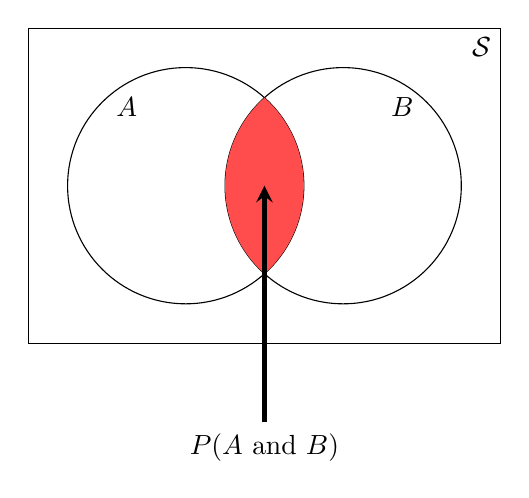
\begin{tikzpicture}
\def\circleA{(2,2) circle [radius = 1.5cm]} 
\def\circleB{(4,2) circle [radius = 1.5cm]} 
\draw (0,0) rectangle (6,4) node [below left] {$\mathcal{S}$};
\draw \circleA;
\node at (1.25,3) {$A$};
\draw \circleB;
\node at (4.75,3) {$B$};
\begin{scope}
\clip \circleA;
\fill[red!70] \circleB;
\end{scope}
\draw [<-, >=stealth, ultra thick] (3,2) -- (3,-1) node [below] {$P(A\text{ and } B)$};
\end{tikzpicture}
\end{center}
\end{frame}

\begin{frame}{Venn Diagram -- AND}
\begin{center}
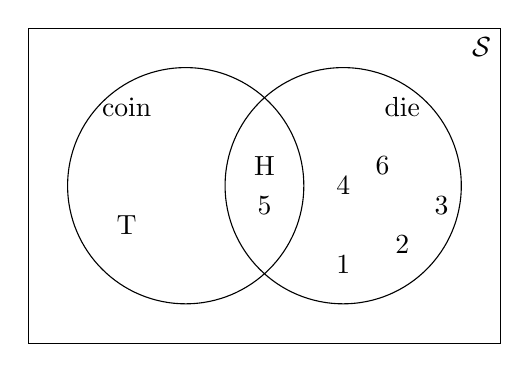
\begin{tikzpicture}
\def\circleA{(2,2) circle [radius = 1.5cm]} 
\def\circleB{(4,2) circle [radius = 1.5cm]} 
\draw (0,0) rectangle (6,4) node [below left] {$\mathcal{S}$};
\draw \circleA;
\node at (1.25,3) {coin};
\draw \circleB;
\node at (4.75,3) {die};
\node at (1.25,1.5) {T};
\node at (3,2.25) {H};
\node at (3,1.75) {5};
\node at (4,1) {1};
\node at (4.75,1.25) {2};
\node at (5.25,1.75) {3};
\node at (4,2) {4};
\node at (4.5,2.25) {6};
\end{tikzpicture}
\end{center}
\end{frame}

\begin{frame}{Tree Diagram}
\begin{center}
\tikzstyle{level 1} = [level distance = 3cm, sibling distance = 10cm]
\tikzstyle{level 2} = [level distance = 3cm, sibling distance = 1.25cm]
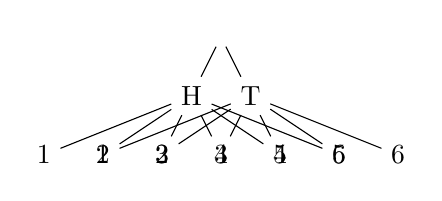
\begin{tikzpicture}[scale=0.5]
\node {}
	child {node {H}
		child {node {1}}
		child {node {2}}
		child {node {3}}
		child {node {4}}
		child {node {5}}
		child {node {6}}}
	child {node {T}{
		child {node {1}}
		child {node {2}}
		child {node {3}}
		child {node {4}}
		child {node {5}}
		child {node {6}} }
		};
\end{tikzpicture}
\end{center}
\end{frame}

% Multiplication Rule
% Tree Diagram
% Mutually Exclusive Events
% Independent vs. Dependent Events
% Conditional Probability

\end{document}
